\documentclass{anstrans}
%%%%%%%%%%%%%%%%%%%%%%%%%%%%%%%%%%%%%%%%%%%%%%%%%%
\title{Leveraging Intel's Embree for Ray Tracing in the DAGMC Toolkit}
\author{Patrick C. Shriwise, Andrew Davis, Paul P.H. Wilson}

\institute{Department of Engineering Physics, University of Wisconsin-Madison, 1500 Engineering Dr, Madison, WI 53706, shriwise@wisc.edu}



%%%%% packages and defs
\usepackage{graphicx}
\usepackage{epsfig}
\usepackage{float}
\usepackage{booktabs}
\usepackage[font={small,it}]{caption}

\begin{document}
%%%%%%%%%%%%%%%%%%%%%%%%%%%%%%%%%%%%%%%%%%%%%%%%%%
\section{Introduction}

The Direct Accelerated Geometry Monte Carlo (DAGMC) \cite{dagmc_2009} toolkit uses the Mesh-Oriented datABase (MOAB) \cite{moab} for the performing geometric operations of Monte Carlo transport on CAD-based geometries. Ray-based operations such as point inclusion, next surface intersection, and surface normal determination are performed on nearly identical geometries to the native geometry of its supported physics engines with all the advantages of the design tools available in CAD software packages.

Analysis using CAD-based geometry has saved man-hours in dealing with tedious and time-consuming geometric design methods, such as text-based geometry, at the cost of additional computational time. Efforts from developers at Intel are opening a pathway to a substantial decrease in this computational cost, leaving only the benefit of reduced human time and effort in the use of CAD-based geometries for Monte Carlo analysis. 

This paper contains the preliminary results for an implementation of Intel's CPU-based ray tracing engine, Embree \cite{embree}, within DagMC for analysis with MCNP5 \cite{mcnp5} on several simple models, some specifically chosen for their complexity in the context of a ray tracing problem.

%%%%%%%%%%%%%%%%%%%%%%%%%%%%%%%%%%%%%%%%%%%%%%%%%%
\section{Spatial Partitioning Trees}

Spatial partitioning trees recursively subdivide the space bounded by a given set of geometric primitives (in our case, triangles) to quickly eliminate regions of the problem space irrelevant to the given ray query for the tree. These subdivisions come in many forms depending on the tree hierarchy being used. These are usually, but not always, binary trees in which each node in the tree has exactly two children with the exception of leaf nodes.

\subsection{Bounding Volume Hierarchies}

%%Bounding volume hierarchies (BVHs) are a subset of a more general solution to the problem of a computational search for a point in 3D space known as spatial partitioning trees. 
In the bounding volume hierarchy (BVH), some volume is used to enclose these regions of 3D space, eventually leading to a subset of triangles to be queried directly for the desired geometric information contained in the leaf nodes of the tree. The most common BVHs use either oriented bounding boxes (OBBs) or axis-aligned bounding boxes (AABBs). AABBs will not conform as tightly to a generic set of data as OBBs. This lack of conformity can lead to increased inefficiency in the tree due to the overlapping of empty space for sibling bounding boxes which results in superfluous node visits. There is an additional cost, however, in using OBBs as bounding volumes. The transformation cost of the ray coordinates from the global problem axes to the local OBB axes for the box intersection check is considerable as this is done many times per ray query. 

\subsection{Other Tree Hierarchies} 

Other bounding volumes and splitting conventions are also used in the area of spatial partitioning trees, for example, bounding spheres are sometimes used rather than boxes due to the simple and fast intersection check needed for ray queries. Hyperplane and hyperplane intervals are also used along each axis to subdivide the problem space into a hierarchical structure similar to that of the BVH. MOAB and Embree both use a BVH with bounding boxes so a detailed discussion of other spatial tree hierarchies will be omitted here.

%%%%%%%%%%%%%%%%%%%%%%%%%%%%%%%%%%%%%%%%%%%%%%%%%%
\section{Intel's Embree}

Many existing ray tracing kernels use fine-grained, data dependent branching and irregular memory access which rules out other, more powerful optimizations like auto-vectorization and parallel tree traversal. Embree's aim is to provide a CPU-based ray tracing kernel which combines the most efficient algorithms, data structures, and parallelization strategies for a given target architecture. Embree aims do do this for modern x86 architectures in order to access their full compute capability. In order to achieve this goal, Embree uses data structures and spatial splitting heuristics that allow for vectorization and parallelization of spatial data structure traversals.

\subsection{Quad-Branching Mixed BVH Traversal}

Most BVHs are implemented as binary trees. Embree, however, uses a quad-branching tree (BVH4) in which each tree node has four children, again, with the exception of leaf nodes. While this increases the number of total nodes in the tree, Embree vectorizes the checking of these nodes, allowing for a larger exclusion of space in about the same time it would take for a check of two nodes in serial execution. 

Embree also employs what is referred to as a mixed tree. A mixed tree indicates the use of multiple bounding volumes. In particular, Embree uses the OBB and AABB mentioned previously. In tree construction, AABBs are used to bound primitives only when deemed appropriate by determining if the local orientation of the triangles are closely aligned with the global axes of the problem space through analysis using interpolated Bezier patches of the primitives to be enclosed.

\subsection{Surface Area Heuristic}

There are many heuristics to be used when partitioning the space contained by a bounding volume. In the past, most BVHs using bounding boxes have used median planar splitting upon construction. This planar splitting is usually done such that the ratio of surface area to volume is maximized (i.e. the volumes are kept as cubic as possible) and the number of contained primitives is being split approximately in half to maintain performance like that of a standard binary tree search in the number of total primitives being contained. 

Recently there has been a new heuristic for partitioning bounding volumes and contained geometric primitives called the surface area heuristic (SAH) \cite{sah}. Given the estimated cost of a single primitive intersection check, this heuristic is designed to minimize the estimated cost of a node split using the number of primitives assigned to each resulting child. Each child term is weighted by the ratio of the child's box area to the parent box area. The ratio of these areas acts as an estimate for the probability of intersection with the child if the parent box is visited during the traversal of the tree. The cost of split is then compared to the node cost as it currently exists. This cost is based purely on the number of primitves the parent box contains multiplied by the estimated intersection check time.

%% This heuristic is designed to minimize the cost $C$ of a split based on the number of primitives to be checked in each child, $P_{R}$ and $P_{L}$, at the cost, $C_{i}$, of a single primitive intersection check weighted by the size of the child boxes, $B_{r}$ and $B_{L}$, compared to the size of the parent box, $B$. There is an additional cost of the extra bounding volume intersection check implied by adding the cost of one traversal step down the tree, $C_{t}$.
%% Its formulation for a binary tree is as follows: 

%% \begin{equation} 
%% C = C_{t} + \frac{SA(B_{L})}{SA(B)} |P_{L}|C_{i} +  \frac{SA(B_{R})}{SA(B)} |P_{R}|C_{i}
%% \end{equation}

One can imagine this heuristic expanded to accommodate the quad-tree in Embree by using additional child terms identical to those of the children represented in the binary tree case. MOAB uses the older method of median planar splitting while Embree uses the SAH in building its mixed BVH4 tree. 

\subsection{Floating Point Precision}

One aspect of Embree's speed is due to the use of float-precision rather than double-precision in its calculations. Currently, this is not typical of ray tracing systems used for scientific Monte Carlo analysis. However, for the sample cases tested for the purpose of this paper, the difference in precision does not necessarily manifest itself in the results. In the future, it is very likely that a double-precision version of Embree will exist via efforts from researchers at the Rensselear Polytechnic Institute \cite{gpu_mic_ray_tracing_rpi}, thus alleviating any concern related to differences in results due to ray tracing calculations.

%%%%%%%%%%%%%%%%%%%%%%%%%%%%%%%%%%%%%%%%%%%%%%%%%%
\section{Implementation of Embree in DagMC}

Embree has been used in DagMC to replace the necessary ray tracing based calculations for use in DagMCNP. The resulting system has been dubbed EmDagMC for the purpose of this paper. 

The implementation began by translating the mesh representation of the geometry in MOAB to an Embree instance. In Embree's native form, the ability to represent the underlying topological structure of a geometry-based mesh is limited in comparison to MOAB. The general topology of Embree's ray tracing kernel is based on 'scenes.'  Each scene is allowed to contain multiple 'geometries' (meshes). That being said, Embree's native topological system does allow for a one-to-one mapping of Embree geometries to MOAB surfaces and Embree scenes to MOAB volumes. This mapping provides DagMC with all the information needed to perform geometric operations required by the various Monte Carlo codes it supports, but in an agnostic manner to the ray tracing kernel being used. Scenes do not share storage of mesh data, so surfaces are reproduced in this system for each volume they belong to. The duplication of surface meshes does have its advantages, however, as triangle normals in MOAB are adjusted on the fly based on which volume a current ray is being fired in while the triangle normals can be pre-adjusted when creating the Embree geometries. This saves several computational steps in many common ray tracing operations found in DagMC. Fortunately, Embree's duplicate mesh representation does not increase the memory footprint of EmDagMC greatly. Even if that were the case, once the Embree mesh representation has been properly established, the MOAB mesh could theoretically be removed from memory to mitigate this problem
.
\begin{figure}

  \begin{center}

    \epsfig{file=figs/sphere.ps,width=.3\columnwidth}
    \epsfig{file=figs/ds.ps,width=.3\columnwidth}
    \epsfig{file=figs/larcyl.ps,width=.3\columnwidth}
    \caption{CAD representations of the sphere, slotted sphere, and high aspect ratio cylinder test models used for ray fire timings of DagMC and EmDagMC. (left to right) \label{models}}

  \end{center}
\vspace{-0.3cm}

\end{figure} 

In DagMC, particles on or just outside the surface of a volume are handled by ignoring the near-surface intersection upon entering a new volume. Under the convention that triangle normals point outward from the center of the volume, this is done by ignoring triangles with normals opposing the current ray direction via a dot product calculation. In Embree, filter functions are used to emulate this process. Filter functions in Embree allow for a user-defined callback function for ray intersections. Embree will return its most recent valid intersection with all associated ray data (the hit triangle's unnormalized normal vector included) and allow a user to determine whether or not to accept the hit or instruct Embree to continue the ray based on the outcome of the said filter function. Thus this calculation is actually contained within the ray query process in EmDagMC as it is in DagMC.

%% \subsection{Support for other applications}

%% Some spatial search operations needed by applications other than MCNP to be fully supported in DagMC are not natively supported by Embree, but due to Embree's allowance of direct access to their spatial tree structures, these functions can easily be implemented in a similar way to current ray intersection functions in Embree. In particular, this involves the implementation of a function for returning the closest point on a volume mesh to a given point in space.

\subsection{Ray Fire Timing: DagMC vs. EmDagMC}

Several single-volume models have become the standard for testing ray fire timing of DagMC. These models include a single sphere, a sphere with notches cut into it, and a high-aspect ratio cylinder all centered on the origin (Figure \ref{models}) . In testing, each of these models are meshed using increasingly smaller faceting tolerances to vary the number of triangles in the problem. The faceting tolerance is defined as the maximum distance between the faceted (meshed) curve or surface and the geometric curve or surface it resolves. 600,000 rays are fired from the origin of the geometry with an isotropic distribution in direction using the same random number seed to ensure consistency of the ray fire timing for both ray fire systems.

\begin{figure}

  \begin{center}

    \epsfig{file=figs/hv.ps,width=.5\columnwidth}
    \caption{Example of the high-valence regions found in the slotted sphere at a high faceting tolerance (1e-04 cm) \label{hv}}

  \end{center}

\end{figure}

Each model presents its own challenge with increasing faceting tolerance. The sphere is a brute force test case. The number of triangles in the generated spherical mesh will always increase with decreasing faceting tolerance. This is not true of some geometries such as cubes or other rectangular parallelepipeds. In the case of the notched sphere, regions referred to as ``high-valence'' are generated as a result of faceting algorithms for planar surfaces meeting curved surfaces. High-valence regions are defined as a single vertex connected to a high number of triangles (Figure \ref{hv}). High-valency is a difficult problem for BHVs to handle. The high triangle density at low faceting tolerances usually results in large overlaps in the bounding volumes of the tree leading to inefficient tree traversals upon query. The faceting of the high aspect ratio cylinder will contain many small, thin triangles running along the barrel of the cylinder. In similar fashion to the spherical model, the number of these triangles will continually increase with decreasing faceting tolerance, resulting in an increasing triangle density as well. The particular shape of these triangles can cause problems in the calculations of tightly fitting OBBs used in DagMC to create spatial trees. This test model is used to determine the overall effectiveness of Embree's ability to use both OBBs and AABBs as well as the robustness of their OBB generation algorithms for fitting to geometric objects with surface meshes of this nature.

DagMC ray fire tests were performed for faceting tolerances ranging from 1e-06 cm to 1e-01 cm on each model. The number of triangles in each problem ranges from thousands to tens of millions of triangles. It should be noted that this will affect the faceting of some models more than others, but the upward trend in the pure number of triangles with decreasing faceting tolerance will be consistent among them all due to the presence of curved surfaces in all test models. Figure \ref{rftiming} shows the results of these tests. A direct model to model comparison indicates that EmDagMC's average ray fire times are approximately 100 times faster than DagMC's. Comparing the best average ray fire time of DagMC to the worst of EmDagMC still leaves DagMC 10 times slower than EmDagMC. There are many operations in DagMC which lie outside the realm of the ray tracing, but these results indicate that the limitation of DagMC's speed due to ray tracing may easily be removed through the use of Embree.

\subsection{Application of EmDagMC with MCNP5}

Several simple models were used to verify that MCNP, DagMCNP and EmDagMCNP provide answers within reason of each other. These models included a sphere, a cube, a set of nested spheres, and a set of nested cubes (3 volumes in each nested case) all filled with a dense hydrogen material for high collisionality in the problem. All of the Monte Carlo models were faceted using a tolerance of 1e-04 cm. A 5 MeV neutron source was placed at the origin, and one million particles were run in each test.


\begin{figure}[H]

  \begin{center}
    
    \epsfig{file=figs/moab_rf.ps,width=0.9\columnwidth}
    \epsfig{file=figs/embree_rf.ps,width=0.9\columnwidth}
    \caption{Comparison of the average ray fire times for MOAB to Embree in all test models. Note the value of the exponent on the y-axis in each graph. \label{rftiming}}
    
  \end{center}

\end{figure}

As expected, the native MCNP runs were generally the fastest with the exception of the nested cubes case in which EmDagMCNP outperformed MCNP by 8 percent (see Table \ref{timings}). This is likely due to the fact that there are very few triangles in the faceted representation of a cube, but there are many surfaces. MCNP searches linearly through a cell's surfaces to find the next surface intersection whereas DagMCNP and EmDagMCNP both search spatially. In the case of the nested cubes, it is likely that the number of surfaces relative to the number of triangles in this problem was high enough to allow EmDagMCNP ray tracing kernel to overtake MCNP's geometric calculations.

\begin{table}
  \small
  \begin{center}

      \caption{Computational Time Comparison}
      \label{timings}
    \begin{tabular}{lccc}



      \toprule
      Test Model & MCNP & DagMCNP & EmDagMCNP \\
      %%\hline
      & \multicolumn{3}{c}{\textbf{time (min)}} \\
      \hline
      Sphere & 2.93 & 25.13 & 4.73  \\
      Cube & 5.03 & 10.56  & 5.80 \\
      Nested Spheres & 4.35 & 50.82 & 7.94 \\
      Nested Cubes & 4.73 & 9.26 & 4.35 \\
      %%\hline
      &  \multicolumn{3}{c}{\textbf{histories/min}} \\
      \hline
      Sphere & 3.4104E+05  & 3.9944E+04  & 2.1810E+05   \\
      Cube & 1.9879E+05 & 9.4738E+04 & 1.7260E+05 \\
      Nested Spheres & 2.2991E+05 & 1.9877E+04 & 1.3947E+05 \\
      Nested Cubes & 2.1170E+05 & 1.0806E+05 & 2.3026E+05 \\
      \bottomrule
      
    \end{tabular}
  \end{center}
\end{table}

%% MCNP's calculated figure of merit (FOM) for each tally varies significantly between MCNP, EmDagMCNP, and DagMCNP. Generally, the FOM values for native MCNP and EmDagMCNP were an order of magnitude higher than DagMC. This is largely due to the fact that the FOM calculation is proportional to the number of histories run per minute. This is indicative of why DagMCNP's FOM values are lower than the MCNP or EmDagMCNP.

%% \begin{table}[h]

%%   \begin{center}
%%     \caption{Single Sphere Timing and Tally Results}

%%     \begin{tabular}{lccc}
%%       \toprule
%%       Value & MCNP & DagMCNP & w/ EmDagMCNP \\
%%       \toprule
%%       %%Hist/min & 3.4104E+05  & 3.9944E+04  & 2.1810E+05  \\
%%       %%\hline
%%       \multicolumn{4}{l}{\textbf{Flux}  ($cm^{-2}$) } \\
%%       \hline
%%       Tally & 4.98083E-03 & 4.98090E-03 & 4.98090E-03 \\
%%       Err & 4E-4 & 4E-4 & 4E-4  \\
%%       FOM & 2.47231E+06 & 2.89558E+05 & 1.58107E+06 \\
%%       \hline
%%       \multicolumn{4}{l}{\textbf{Energy} (MeV/g)} \\
%%       \hline
%%       Tally & 3.17819E-03 & 3.17824E-03 & 3.17824E-03 \\
%%       Err & 5E-4 & 5E-4 & 5E-4 \\
%%       FOM & 1.16162E+06 & 1.36051E+05 & 7.42879E+05 \\      
%%       \bottomrule
                        
%%     \end{tabular}


%%   \end{center}

%% \end{table}


%% \begin{table}[h]

%%   \begin{center}
%%     \caption{Single Cube Timing and Tally Results}

%%     \begin{tabular}{lccc}
%%      \toprule
%%       Value & MCNP & DagMCNP & w/ EmDagMCNP \\
%%      \toprule
%%      %%Hist/min & 1.9879E+05 & 9.4738E+04 & 1.7260E+05  \\
%%      %%\hline
%%      \multicolumn{4}{l}{\textbf{Flux} ($cm^{-2}$)} \\
%%      \hline
%%      Tally & 5.61374E-03 & 5.61374E-03 & 5.61374E-03 \\
%%      Err & 3E-4 & 3E-4 & 3E-4  \\
%%      FOM & 2.47008E+06 & 1.17719E+06 & 2.14469E+06 \\
%%      \hline
%%      \multicolumn{4}{l}{\textbf{Energy} (MeV/g)} \\
%%      \hline
%%      Tally & 2.98933E-03 & 2.98933E-03 & 2.98933E-03 \\
%%      Err & 7E-4 & 7E-4 & 7E-4 \\
%%      FOM & 3.99526E+05 & 1.90406E+05 & 3.46895E+05 \\
%%      \bottomrule
     
%%     \end{tabular}


%%   \end{center}
%% \vspace{-0.4cm}
%% \end{table}

In the single volume test cases, the flux and energy tallies from native MCNP differ from both of the DagMC-based implementations slightly, but both of the ray tracing methods agreed with each other exactly. The tally errors were identical across all three systems for the single volume test cases. The multiple volume test results (see Tables \ref{nestedspheres} and \ref{nestedcubes}) showed similar trends to the single volume tests with the exception of a discrepancy between DagMC and EmDagMC in the flux tally of the outermost cell, cell 3, in the nested spheres model. Based on the number of tracks entering each cell, this appears to be caused by a single particle history in EmDagMCNP ending before a surface in cell 2 while in DagMCNP it crosses into cell 3 before dying. It is believed that the discrepancy is the result of a systematic difference between Embree and MOAB's ray fire conventionality rather than the result of Embree's use of floating point precision, but the latter possibility has not yet been ruled out.

\begin{table}
  \small
  \begin{center}
    \caption{Nested Spheres Timing and Tally Results. Flux tally units are $cm^{-2}$. Energy tally units are MeV/g.}
    \label{nestedspheres}
    \begin{tabular}{lccc}
      \toprule
      Value & MCNP & DagMCNP & EmDagMCNP \\
      \toprule
      %%Hist/min & 2.2991E+05 & 1.9877E+04 & 1.3947E+05 \\
      %%\hline
      \multicolumn{4}{l}{\textbf{Cell 1 Tallies}} \\
      \hline
      Flux  & 5.25725E-03 & 5.25734E-03 & 5.25734E-03 \\
      Energy  & 3.17869E-03 &  3.17873E-03 &  3.17873E-03 \\
      \hline
      \multicolumn{4}{l}{\textbf{Cell 2 Tallies}} \\
      \hline
      Flux  & 1.91645E-04 & 1.91644E-04 & 1.91644E-04 \\
      Energy  & 5.22131E-05 & 5.22137E-05 & 5.22137E-05 \\
      \hline
      \multicolumn{4}{l}{\textbf{Cell 3 Tallies}} \\
      \hline
      Flux  & 1.18371E-05 & 1.18376E-05 & 1.18410E-05 \\
      Energy  & 4.96282E-06 & 4.96285E-06 & 4.96285E-06 \\
      \bottomrule
                        
    \end{tabular}


  \end{center}
%%\vspace{-0.2cm}
\end{table}


\begin{table}
  \small
  \begin{center}
    \caption{Nested Cubes Timing and Tally Results. Flux tally units are $cm^{-2}$. Energy tally units are MeV/g.  }
    \label{nestedcubes}
    \begin{tabular}{lccc}
      \toprule
      Value & MCNP & DagMCNP & EmDagMCNP \\
      \toprule
      %%Hist/min & 2.1170E+05 & 1.0806E+05 & 2.3026E+05 \\
      %%\hline
      \multicolumn{4}{l}{\textbf{Cell 1 Tallies}} \\
      \hline
      Flux  & 1.38556E-02 & 1.38556E-02 & 1.38556E-02 \\
      Energy  & 1.05974E-02 & 1.05974E-02 & 1.05974E-02 \\
      \hline
      \multicolumn{4}{l}{\textbf{Cell 2 Tallies}} \\
      \hline
      Flux  & 1.41609E-03 & 1.41609E-03 & 1.41609E-03 \\
      Energy  & 4.81169E-04 & 4.81169E-04 & 4.81169E-04 \\
      \hline
      \multicolumn{4}{l}{\textbf{Cell 3 Tallies}} \\
      \hline
      Flux  & 1.92847E-04 & 1.92847E-04 & 1.92847E-04 \\
      Energy  & 1.10361E-04 & 1.10361E-04 & 1.10361E-04 \\
      \bottomrule
      
                        
    \end{tabular}


  \end{center}
%%\vspace{-0.2 cm}
\end{table}

It is worth noting that no particles were lost in any of the test runs presented here. The full robustness of DagMC's topologically watertight meshes is available to the Embree instance in combination with Embree's own floating point watertight triangle intersection algorithm.  \cite{make_watertight_smith_2010} \cite{watertight_tri_intersection_woop_2013} As a result, we expect the lost particle rate to match that of DagMC for any watertight model. 

\section{Conclusions and Future Work}

The implementation of a highly efficient CPU-based ray tracing system, Intel's Embree, in DagMC has been demonstrated in this paper. A small, and likely systematic, discrepancy between the MOAB ray tracing system and Embree has yet to be resolved, but the possibility of CAD-based MCNP simulations being able to run on the order of simulations using native MCNP geometry has been shown.
In the future, test cases on more complex CAD models will be attempted using the EmDagMC system for proof of application to real world problem scenarios. Pending the success of these tests, the DagMC build system will temporarily be redesigned to support Embree as the underlying ray tracing system if specified by the user. In the long term, the goal of this work will be to develop an equally efficient ray tracing system in MOAB using its direct access capabilities to take advantage of some of the same optimizations as Embree, but with design considerations for a more diverse set of spatial tree structures in mind. 

\vspace{-0.2cm}
\bibliographystyle{ans}
\bibliography{bibliography}


\end{document}
